\documentclass[a4paper]{article}

\usepackage[english]{babel}
\usepackage[utf8]{inputenc}
\usepackage{graphicx}
\usepackage{enumitem}
\usepackage{blindtext}

\usepackage{amsmath}

\graphicspath{ {./images/} }
\setlength\parindent{0pt}
    
\title{CS2500 Project 3 \\ 0-1 Knapsack}
\author{Evan Wilcox}
\date{Due April 4, 2019}


\begin{document}
    \maketitle

    \section{Motivation}
    The 0-1 knapsack is a classic optimization problem in computer science. Optimization 
    problems can be seen in everyday life such as a CPU scheduler, a delivery route planner, 
    or a car's brake controller. All of these problems have a solution but usually that 
    solution is costly to generate. Developers instead create an algorithm that will generate
    an approximate solution but in much less time. Your trading accuracy for time. This report
    will analyse two algorithms and their approximate equivalent to determine the benefit of 
    this trade off.


    \section{Background}
    In the 0-1 knapsack problem you are given a set of items each with a weight, $w_{i}$,
    and a value, $v_{i}$. The goal is to put a combination of items in a knapsack 
    that has a capacity $W$ that maximizes the profit of the items in the knapsack. \\

    One solution to the 0-1 knapsack is implementing its recurrence directly into 
    code using recursion. The recurrence is as follows:
    
    \[ f(i, W)=\begin{cases} 
      \text{max}\{f(i-1, W), f(i-1, W-w_{i}) + v_{i}\}\\
      f(i-1, W) \\
    \end{cases}
    \]

    with $i$ being the number of items. Implemeting the recurrence directly in code
    will give you the solution but is very slow running in $2^{n}$ time because it 
    recomputes subproblems many times over. \\ 

    The recurrence can also be implemented iteratively. Using a 2d array you can store
    solutions to subproblems as you go so they only have to be computed once. This 
    method will provide the same solution as the above recurrence but will run in 
    linear time. \\


    Another approach is the greedy method. The greedy method first sorts the 
    items in decreasing order by its value per weight, $v_{i}/w_{i}$. The greedy 
    algorithm proceeds to add the items to the knapsack unless the item won't fit or
    until the bag is full. Because this approach makes "greedy" choices, it is not a 
    solution to the 0-1 knapsack but instead a close approximation. Even though he 
    greedy algorithm runs in linear time making only one decision for each item, add 
    the item or don't, it must first sort the items which runs in $n$lg$n$ time. \\



    \section{Procedures}
    \begin{enumerate}

        \item Express the three approaches in pseudocode.

        \item Implement the three algorithms in c++.
        
        \item Measure run times of the three algorithms to experimentally determine 
              their run time complexity and compare to their expected run time 
              complexity.

        \item Develop and implement a testing plan.
        
        \item List problems encountered during development.
        
        \item Produce a conclusion addressing the efficacy of the methods used.
    \end{enumerate}

    
    \section{Pseudocode}
    \textbf{Recursive Knapsack} \\
    1 knapSack$(W, n)$ \\
    2 if $n == 0$ or $W == 0$ \\
    3   \phantom{hell}return 0 \\
    4 
    5 if $wt[n-1] > W$ \\
    6 \phantom{hell}return knapSack$(W, wt, val, n-1)$ \\
    7 else \\
    8 \phantom{hell}return MAX\{val$[n-1]$ + knapSack$(W-wt[n-1], wt, val, n-1)$, \\
                              \phantom{hellhellhellhellhell}knapSack$(W, wt, val, n-1)$\} \\

    \textbf{Iterative Knapsack} \\
    iterativeKnapSack$(W, n)$ \\
    1 new 2d array $K[n+1][W+1]$ \\
    2 \\
    3 for $i = 1$ to $n$ \\
    4 \phantom{hell}for $w = 1$ to $w$ \\
    5 \phantom{hellhell}if $i == 0$ or $w == 0$ \\
    6 \phantom{hellhellhell}$K[i][w] = 0$ \\
    7 \phantom{hellhell}else if $wt[i-1] <= w$ \\
    8 \phantom{hellhellhell}$K[i][w] = $MAX$\{val[i-1] + K[i-1][w-wt[i-1]], K[i-1][w]\}$ \\
    9 \phantom{hellhell}else \\
    10 \phantom{hellhellhel}$K[i][w] = K[i-1][w]$ \\
    11 return $K[n][W]$ \\
    
    \newpage
    \textbf{Greedy Knapsack} \\
    1 greedyKnapSack$(W, n)$ \\
    2 \\
    3 sort$(W, wt, val, n)$ \\
    4 for $i = 1$ to $n$ \\
    5 \phantom{hell}if $wt_{i} <= W$ \\
    6 \phantom{hellhell}$profit += val_{i}$ \\
    7 \phantom{hellhell}$W -= wt_{i}$ \\
    8 return $profit$


    \section{Testing Plan}
    All three algorithms were tested with the following testing plan: \\

    \begin{tabular}{ |l|l|}
        \hline
        \textbf{Input} & \textbf{Expected Output}\\ \hline
        Empty array, $n=0$ & Profit of 0 \\ \hline
        $W=0$ & Profit of \\ \hline
    \end{tabular}

    
    \section{Problems Encountered}
    One problem encountered was that the iterative knapsack algorithm hit a segmentation fault
    error when the problem size was greater than about 500. I narrowed this problem down to 
    an error int the method used to allocate the memory used for the 2d array. Also my 
    recursive knapsack algorithm was not finding the best solution until I realised there was
    an error in my recursive case. 

    
    \section{Performance Results} 
    After testing each algorithm with varying sets of data, all three algorithms 
    followed their expected run time complexity. The recursive knapsack algorithm 
    started to show its expected runtime of $2^{n}$ at around $n \approx 100$. 
    \begin{center}
      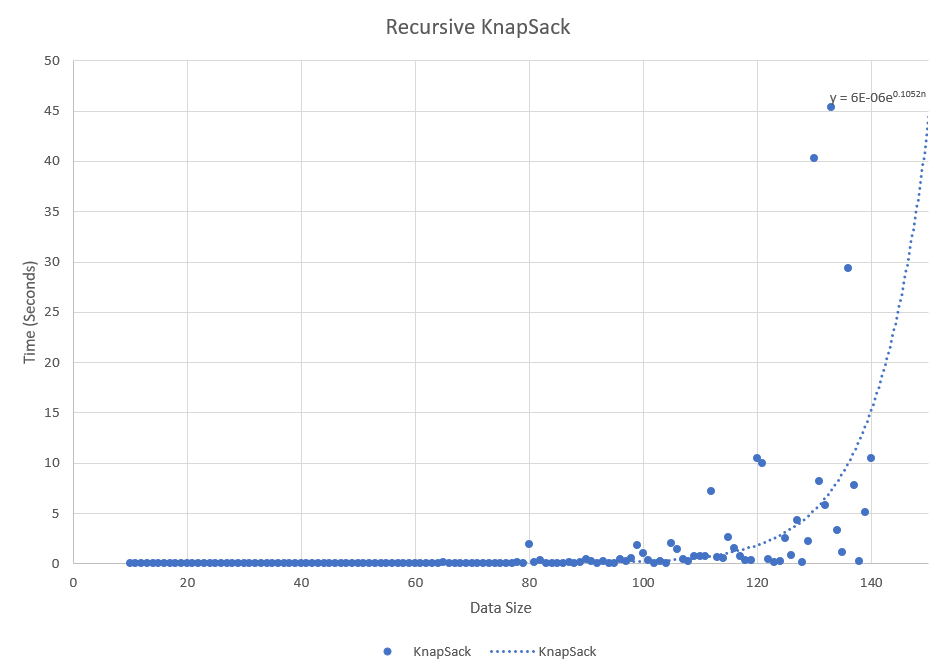
\includegraphics[scale=0.6]{1} \\
    \end{center}

    The greedy approach actually ended up having a lower average run time than the
    iterative version even though the iterative version has a better runtime complexity
    of $n$ vs. the greedy method's $n$lg$n$. Both algorithms started showing their 
    runtime complexities at around $n \approx 10$.
    \begin{center}
      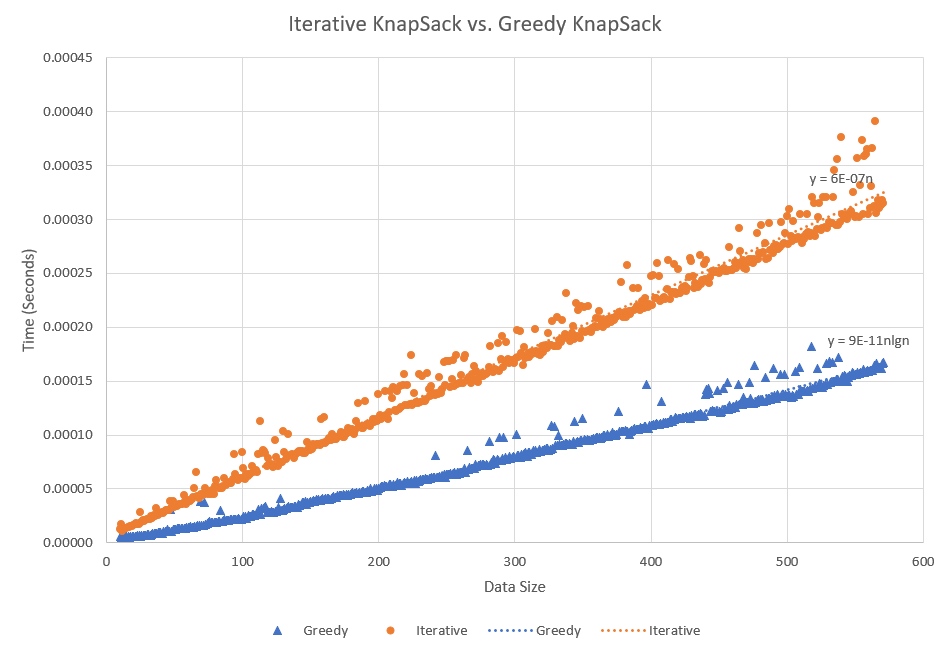
\includegraphics[scale=0.6]{2} \\
    \end{center}


    \section{Conclusion}
    Both the recursive and iterative versions of the 0-1 knapsack will provide the 
    correct solution to the given data set with the iterative version doing it much
    faster because of it's linear complexity. However, the greedy algorithm beat 
    the iterative algorithm despite it's worse expected runtime complexity. I suspect
    this is because even though the greedy algorithm needs to sort the items the 
    amount of items being sorted is relatively small so it doesn't contribute much
    to the overall runtime. Also the iterative algorithm used in testing dynamically
    allocates a 2d array to store the solutions to the subproblems while the greedy 
    version doesn't allocate any new memory. \\

    In conclusion, if you want the solution to the 0-1 knapsack you should use the 
    iterative version because it is the fastest way to always get the solution. But 
    if you are okay with a small margin of error, the greedy version will generate 
    an approximate solution faster than the iterative version will generate the full
    solution.


    \newpage
    \textbf{Appendix A} - Source Code
    \begin{verbatim}
/*
* Author: Evan Wilcox
* File: main.cpp Date: 4/4/2019
* Class: CS 2500 Sec. 1
* Instructor : Bruce McMillin
* Main file for Project 3
*/

#include <iostream>
#include <fstream>
#include "knapSack.h"
#include <time.h>
using namespace std;


int main()
{
  ofstream fout;
  fout.open("out.csv");
  
  const int MAX = 100000;

  int val[MAX];
  int wt[MAX];

  Item arr[MAX];
  int W = 50;

  clock_t t;
  fout << "N," << "KnapSack," << "Greedy," << "Iterative," << endl;

  int n;
  for(n = 10; n < MAX; n++)
  {
    for(int i = 0; i < n; i++)
    {
      int v = (rand() % 100) + 51;
      int w = (rand() % 50) + 1;

      val[i] = v;
      wt[i] = w;

      arr[i].m_val = v;
      arr[i].m_wt = w;
    }

    fout << n << ",";
    cout << n << endl;

    t = clock();
    knapSack(W, wt, val, n);
    fout << (float)(clock()-t)/CLOCKS_PER_SEC << ",";

    t = clock();
    greedyKnapSack(W, arr, n);
    fout << (float)(clock()-t)/CLOCKS_PER_SEC << ",";

    t = clock();
    iterativeKnapSack(W, wt, val, n);
    fout << (float)(clock()-t)/CLOCKS_PER_SEC;

    fout << endl;
  }

  fout.close();

  return 0;
}

/*
* Author: Evan Wilcox
* File: knapSack.h Date: 4/4/2019
* Class: CS 2500 Sec. 1
* Instructor : Bruce McMillin
* Header file for knapSack.cpp
*/

#ifndef KNAPSACK_H
#define KNAPSACK_H

using namespace std;

/*
* Struct: Item
* A pairing of an item's weight and value.
*/
struct Item
{
  int m_val;
  int m_wt;

  Item(int val, int wt) : m_val(val), m_wt(wt){}
  Item() : m_val(0), m_wt(0){}
};

/*
* Function: compare
* Description: function used to compare two items by their m_val/m_wt
* Pre: a.m_wt != 0 and b.m_wt != 0
* Post: an int is returned
* Param a : an item
* Param b : an item
* Return:  1 if a's m_val/m_wt is less than b's,
          -1 if b's m_val/m_wt is greater than a's,
           0 if they are equal
*/
int compare(const void * a, const void * b);

/*
* Function: greedyKnapSack
* Description: a greedy implementation of the 0-1 knapsack
* Pre: W >= 0, arr[i].m_wt > 0, n >= 0
* Post: arr is sorted by arr[i].m_val/arr[i].m_wt ratio
* Param W : capacity remaining in the knapsack
* Param arr : array of items to try and put in the knapsack
* Param n : index of item in arr to try and put in the knapsack
* Return: greedy approximate to 0-1 knapsack problem
*/
int greedyKnapSack(int W, struct Item arr[], int n);

/*
* Function: knapSack
* Description: recursive implementation of the 0-1 knapsack
* Pre: W >= 0, wt[i] > 0, n >= 0
* Post: none
* Param W : capacity remaining in the knapsack
* Param wt : array of weights of items
* Param val : array of values of items
* Param n : index of item in wt/val to try and put in the knapsack
* Return: solution to knapsack problem
*/
int knapSack(int W, int wt[], int val[], int n);

/*
* Function: iterativeKnapSack
* Description: iterative implementation of the 0-1 knapsack
* Pre: W >= 0, wt[i] > 0, n >= 0
* Post: none
* Param W : capacity remaining in the knapsack
* Param wt : array of weights of items
* Param val : array of values of items
* Param n : index of item in wt/val to try and put in the knapsack
* Return: solution to knapsack problem
*/
int iterativeKnapSack(int W, int wt[], int val[], int n);

/*
* Function: max
* Description: A simple max function
* Pre: none
* Post: an int is returned
* Param a : an int
* Param b : an int
* Return: a if a > b, otherwise b
*/
int max(int a, int b);

#endif

/*
* Author: Evan Wilcox
* File: knapSack.cpp Date: 4/4/2019
* Class: CS 2500 Sec. 1
* Instructor : Bruce McMillin
* Implementation file for three solutions to the 0-1 knapSack
*/

#include "knapSack.h"


int compare(const void * a, const void * b)
{
  double r1 = (double)(*(Item*)a).m_val / (*(Item*)a).m_wt;
  double r2 = (double)(*(Item*)b).m_val / (*(Item*)b).m_wt;

  if( r1 <  r2 )
  {
    return 1;
  } 
  else if( r1 >  r2 ) 
  {
    return -1;
  } 
  else
  {
    return 0;
  }
}


int greedyKnapSack(int W, struct Item arr[], int n)
{
  qsort(arr, n, sizeof(arr[0]), compare);
  
  int curWeight = 0;
  double finalvalue = 0.0;

  for(int i = 0; i < n; i++)
  {
    if(curWeight + arr[i].m_wt <= W)
    {
      curWeight += arr[i].m_wt;
      finalvalue += arr[i].m_val;
    }
  }

  return finalvalue;
}


int knapSack(int W, int wt[], int val[], int n)
{
  if(n == 0 || W == 0)
  {
    return 0;
  }

  if(wt[n-1] > W)
  {
    return knapSack(W, wt, val, n-1);
  }
  else
  {
    return max(val[n-1] + knapSack(W-wt[n-1], wt, val, n-1), knapSack(W, wt, val, n-1));
  }
}


int iterativeKnapSack(int W, int wt[], int val[], int n)
{
  int i, w;

  int** K = new int*[n+1];
  for(int j = 0; j < n+1 ; j++)
  {
    K[j] = new int[W+1];
  }

  for(i = 0; i <= n ; i++)
  {
    for (w = 0; w <= W ; w++)
    {
      if(i == 0 || w == 0)
      {
        K[i][w] = 0;
      }
      else if(wt[i-1] <= w)
      {
        K[i][w] = max(val[i-1] + K[i-1][w-wt[i-1]], K[i-1][w]);
      }
      else
      {
        K[i][w] = K[i-1][w];
      }
    }
  }

  for(int j = 0; j < n+1 ; j++)
  {
    delete K[j];
  }
  delete K;

  return K[n][W];
}


int max(int a, int b)
{
  return (a > b) ? a : b;
}

    \end{verbatim}

\end{document}